% !TeX root = ../tjuthesis-example.tex

\section{排版示例}

这一章中我们给出一些排版示例, 以便一些对\LaTeX 不熟悉的同学来学习参考.

\subsection{插图}

手册中对插图有如下要求:
\begin{enumerate}
  \item 图居中, 上下与正文之间各空一行;
  \item 图中文字: 小五, 宋体 (英文 Times New Roman), 行距1倍, 段前0行, 段后0行
  \item 插图应有图序和图题, 全文插图以章分组编序号, 图序必须连续, 不得重复或跳缺. 如图4.1表示第四章的第一幅图;
  \item 图题: 小五, 宋体 (英文 Times New Roman), 居中置于图下方, 行距18磅, 段前0行, 段后0行.
\end{enumerate}

现在我们应该来说一下应该如何插图. 我们在文档类中已经引用了\pkg{graphicx}包. 我们拿手册中的插图作为示例.

\begin{figure}[htb]
  \centering
  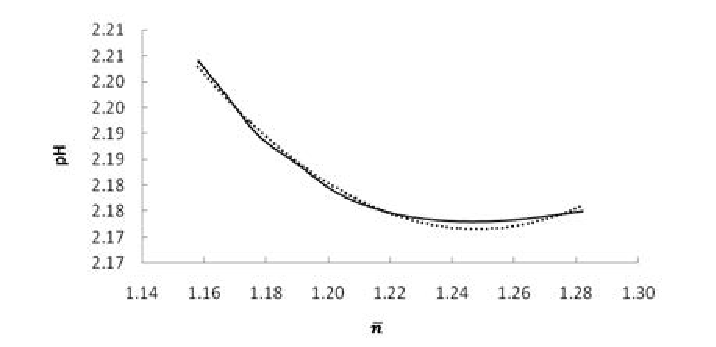
\includegraphics{figures/oxalic-acid-n-geq-1.15.pdf}
  \caption{乙二酸$\overline{n}\geq 1.15$数据段曲线及其拟合曲线 (实线--实际曲线, 虚线--拟合曲线) 乙二酸$\overline{n}\geq 1.15$数据段曲线及其拟合曲线 (实线--实际曲线, 虚线--拟合曲线) 乙二酸$\overline{n}\geq 1.15$数据段曲线及其拟合曲线 (实线--实际曲线, 虚线--拟合曲线)}
\end{figure}

\zhlipsum[1]
